\chapter{METHODOLOGY}
\label{chp:methodology}

\TODO{write}

\section{Approach Overview}
\label{sec:approach-overview}
\TODO{write}
buraya akış şeması çiz

\section{Process Model Mining}
\label{sec:process-model-mining}

Process model mining stage in the proposed approach has the aim of creating reproducible and generalized process models from event logs. In order to achieve this aim, implementation of \textit{Inductive Miner Infrequent (IMi)}, which is proposed in \cite{leemans2014discoveringinfrequent} as an extension to \textit{Inductive Miner} to handle noise in the event logs, is used in this study. 
The selected implementation has the ability of pruning data to handle noise in the event logs. Like the other data mining approaches, event logs include data related to the infrequent behaviors occurred in real life. Although these infrequent behaviors might be caused by important structural or case related issues that should be analyzed; they make the process of mining and results more complex. In the scope of this study, without cleaning the data, most of the process model mining approaches result with \textit{spaghetti-like models}\cite{van2011process} which are difficult to further analyze. Since this thesis focuses on learning from the cross-organizational process mining rather than creating the best-fitting process models, data cleaning and noise handling is a necessary step. Therefore preprocessing steps are undertaken with a compatible approach of \textit{Inductive Miner Infrequent (IMi)}, where data is cleaned in every inductive step.
Considering the scope of this study, instead of computational details of \textit{Inductive Miner Infrequent (IMi)} black-box approach is used to explain its usage in the methodology. In order to provide a filtering threshold, a user-provided value between 0 to 1 is added as input to method with the event logs. As a result, workflow net is produced which is a sound and properly completed Petri net without deadlocks. Black-box of this stage is illustrated in Figure~\ref{fig:process-model-mining-blackbox} and this stage is called for every organization's event logs to create their own process models in Workflow net formalization.

\begin{figure}
  \centering
  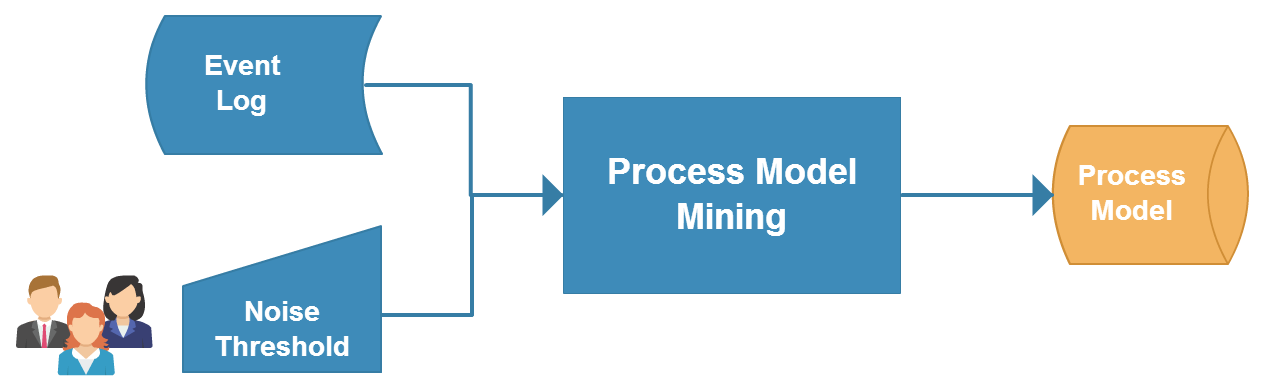
\includegraphics[width=\textwidth]{4_methodology/process-model-mining-blackbox}
  \caption{Process Model Mining Stage as Black-box }
  \label{fig:process-model-mining-blackbox}
\end{figure}


\section{Performance Indicator Analysis}
\label{sec:performance-indicator-analysis}
	Replay
	Performance Summary

\section{Mismatch Pattern Analysis}
\label{sec:mismatch-pattern-analysis}
	BPMN Conversion


\section{Recommendation Generation}
\label{sec:recommendation-generation}



\section{Implementation}
\label{sec:implementation}
buraya arch. çiz
